% 


\documentclass[twoside]{article}
\setlength{\oddsidemargin}{0.25 in}
\setlength{\evensidemargin}{-0.25 in}
\setlength{\topmargin}{-0.6 in}
\setlength{\textwidth}{6.5 in}
\setlength{\textheight}{8.5 in}
\setlength{\headsep}{0.75 in}
\setlength{\parindent}{0 in}
\setlength{\parskip}{0.1 in}

%
% ADD PACKAGES here:
%

\usepackage{amsmath,amsfonts,graphicx,arydshln}


\newcounter{lecnum}
\renewcommand{\thepage}{\thelecnum-\arabic{page}}
\renewcommand{\thesection}{\thelecnum.\arabic{section}}
\renewcommand{\theequation}{\thelecnum.\arabic{equation}}
\renewcommand{\thefigure}{\thelecnum.\arabic{figure}}
\renewcommand{\thetable}{\thelecnum.\arabic{table}}

%
% The following macro is used to generate the header.
%
\newcommand{\lecture}[4]{
   \pagestyle{myheadings}
   \thispagestyle{plain}
   \newpage
   \setcounter{lecnum}{#1}
   \setcounter{page}{1}
   \noindent
   \begin{center}
   \framebox{
      \vbox{\vspace{2mm}
    \hbox to 6.28in { {\bf EE502 - Linear Systems Theory II
	\hfill Spring 2023} }
       \vspace{4mm}
       \hbox to 6.28in { {\Large \hfill Lecture #1 \hfill} }
       \vspace{2mm}
       \hbox to 6.28in { {\it Lecturer: #2 \hfill } }
      \vspace{2mm}}
   }
   \end{center}
   \markboth{Lecture #1}{Lecture #1}

   \vspace*{4mm}
}

\renewcommand{\cite}[1]{[#1]}
\def\beginrefs{\begin{list}%
        {[\arabic{equation}]}{\usecounter{equation}
         \setlength{\leftmargin}{2.0truecm}\setlength{\labelsep}{0.4truecm}%
         \setlength{\labelwidth}{1.6truecm}}}
\def\endrefs{\end{list}}
\def\bibentry#1{\item[\hbox{[#1]}]}


\newcommand{\fig}[3]{
			\vspace{#2}
			\begin{center}
			Figure \thelecnum.#1:~#3
			\end{center}
	}

% Use these for theorems, lemmas, proofs, etc.
\newtheorem{theorem}{Theorem}[lecnum]
\newtheorem{lemma}[theorem]{Lemma}
\newtheorem{proposition}[theorem]{Proposition}
\newtheorem{claim}[theorem]{Claim}
\newtheorem{corollary}[theorem]{Corollary}
\newtheorem{definition}[theorem]{Definition}
\newenvironment{proof}{{\bf Proof:}}{\hfill\rule{2mm}{2mm}}
\newtheorem{exmp}[theorem]{Ex}

% **** IF YOU WANT TO DEFINE ADDITIONAL MACROS FOR YOURSELF, PUT THEM HERE:

\begin{document}

% Lecture Details
\lecture{16}{Asst. Prof. M. Mert Ankarali}

%%%%%%%%%%%%%%%%%%%%%%%%%%

\section{Minimality of Interconnected Systems}

In this section we shall examine the conditions under which minimality is lost when minimal subsystems are interconnected in various configurations,

\subsection{Series - Cascade Connection}
		
Consider the following system structure where two sub systems, with transfer functions 
$G_1(s)$ and $G_2(s)$ and associated minimal representations $\left( \begin{array}{c|c} A_1 & B_1 \\ \hline
C_1 & D_1 \end{array} \right)$ and $\left( \begin{array}{c|c} A_2 & B_2 \\ \hline
C_2 & D_2 \end{array} \right)$, connected in series/cascade configuration. 
		
\begin{center}
  \begin{minipage}[h]{0.9\linewidth}
    \begin{center}
      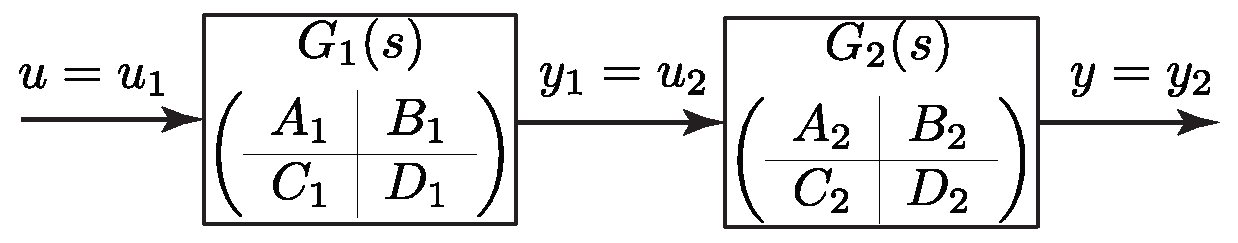
\includegraphics[width=0.8\textwidth]{cascade}
    \end{center}
  \end{minipage}
    \end{center}
		
The transfer function of the connection is simply equal to $G(s) = G_2(s) G_1(s)$. Let $x_1$ and $x_2$
state-variables of the sub-systems, then natural choice of the state variable for the series connection is 
$x = \begin{bmatrix} x_1 \\ x_2 \end{bmatrix}$. Under this definition the state-space representation for the whole system 
can be found as
%
\begin{align*}
A = \left[ \begin{array}{c|c} A_1 & 0 \\ \hline B_2 C_1  & A_2 \end{array} \right]
\, , \, B = \left[ \begin{array}{c} B_1 \\ \hline B_2 D_1  \end{array} \right]
\, , \, C = \left[ \begin{array}{c|c} D_2 C_1 & C_2  \end{array} \right]
\, , \, D = \left[ \begin{array}{c} D_2  D_2  \end{array} \right]
\end{align*}
%
Clearly eigenvalues of A are the combination of the eigenvalues of $A_1$ and $A_2$ and the poles of the system 
Let's analyze the observability of the connection via PBH test. 
%
\begin{align*}
	\left[ \begin{array}{c} \lambda I - A \\ \hline C \end{array} \right]
	= 
	\left[ \begin{array}{c|c} \lambda I - A_1 & 0 \\ \hline -B_2 C_1 &  \lambda I - A_2 \\ \hline 
	D_2 C_1 & C_2
	\end{array} \right]
\end{align*}
%
If we remember from the observability lecture that $(A,C)$ (whole state-space model) pair 
is unobservable if and only if $\left[ \begin{array}{c} \lambda I - A \\ \hline C \end{array} \right]$
losses rank for some $\lambda$, which can only happen if $\lambda$ is an eigenvalue of $A$.
Let's assume that $\lambda_2$ is an eigenvalue of $A_2$ but not eigenvalue of $A_1$. 
Then $\left[ \begin{array}{c} \lambda I - A \\ \hline C \end{array} \right]_{\lambda = \lambda_2}$ 
looses rank, if $\exists v = \begin{bmatrix} v_1 \\ v_2 \end{bmatrix}$ such that 
%
\begin{align*}
	&\left[ \begin{array}{c} \lambda_2 I - A \\ \hline C \end{array} \right] v = 0
	\, \Rightarrow \, 
	\left[ \begin{array}{c|c} \lambda_2 I - A_1 & 0 \\ \hline -B_2 C_1 &  \lambda_2 I - A_2 \\ \hline 
	D_2 C_1 & C_2
	\end{array} \right]  \begin{bmatrix} v_1 \\ v_2 \end{bmatrix} = 0
		\, \Rightarrow \, v_1 = 0 \, \& \, \left[ \begin{array}{c} \lambda_2 I - A \\ \hline C_2 \end{array} \right] v_2 = 0
\end{align*}
%
which contradicts with the fact that $(A_2,C_2)$ is observable since both individual sub-system representations are minimal. 
In that respect $\left[ \begin{array}{c} \lambda I - A \\ \hline C \end{array} \right]$ can loose rank only at an eigenvalue
of $A_1$ (i.e. a pole of $A_2$). Let's $\lambda_1$ is an eigenvalue of $A_1$.
Then $\left[ \begin{array}{c} \lambda I - A \\ \hline C \end{array} \right]_{\lambda = \lambda_1}$ 
looses rank, if $\exists v = \begin{bmatrix} v_1 \\ v_2 \end{bmatrix}$ such that 
%
\begin{align*}
	&\left[ \begin{array}{c} \lambda_1 I - A \\ \hline C \end{array} \right] v = 0
	\, \Rightarrow \, 
	\left[ \begin{array}{c|c} \lambda_1 I - A_1 & 0 \\ \hline -B_2 C_1 &  \lambda_1 I - A_2 \\ \hline 
	D_2 C_1 & C_2
	\end{array} \right]  \begin{bmatrix} v_1 \\ v_2 \end{bmatrix} = 0
		\, \Rightarrow \, v_1 \neq 0 \, \& \, A v_1 = \lambda_1 v_1 \, \mathrm{and}
		\\
	&\left[ \begin{array}{c|c} \lambda_1 I - A_2 & -B_2 C_1 \\ \hline 
	  C_2 & D_2 C_1
	\end{array} \right]  \begin{bmatrix} v_2 \\ v_1 \end{bmatrix} = 0	
	\, \Rightarrow \, 
	\left[ \begin{array}{c|c} \lambda_1 I - A_2 & -B_2  \\ \hline 
	  C_2 & D_2 
	\end{array} \right]  \begin{bmatrix} v_2 \\ C_1 v_1 \end{bmatrix} = 0	
\end{align*}
%
Note that $\left[ \begin{array}{c|c} \lambda_1 I - A_2 & -B_2  \\ \hline 
	  C_2 & D_2 
	\end{array} \right]  \begin{bmatrix} v_2 \\ C_1 v_1 \end{bmatrix} = 0$
implies that $\lambda_1$ is a \textbf{right} zero of $G_2(s)$ where $v_2$ and $C_1 v_1$ 
is the associated \text{state-zero-direction} and \textit{input-zero-direction}
respectively. 

If we summarize the results, cascaded system is unobservable if $\exists (\lambda_1 , v_1)$ and $v_2 \neq 0$
such that $(\lambda_1 , v_1)$ is an eigenvalue-eigenvector pair of $A_1$ and $\lambda_1$ is a \textbf{right} zero of 
$G_2(s)$ with $v_2$ and $C_1 v_1$ as the \text{state-zero-direction} and \textit{input-zero-direction} respectively. 

Now let's analyze the reachability of the connection via PBH test. 
%
\begin{align*}
	\left[ \begin{array}{c|c} \lambda I - A & B \end{array} \right]
	= 
	\left[ \begin{array}{c|c|c} \lambda I - A_1 & 0 & B_1 \\ \hline -B_2 C_1 & \lambda I - A_2 & B_2 D_1 
	\end{array} \right]
\end{align*}
%
If we remember from the reachability lecture that $(A,B)$ (whole state-space model) pair 
is unreachable if and only if $\left[ \begin{array}{c|c} \lambda I - A & B \end{array} \right]$
losses rank for some $\lambda$, which can only happen if $\lambda$ is an eigenvalue of $A$.
Let's assume that $\lambda_1$ is an eigenvalue of $A_1$ but not eigenvalue of $A_2$. 
Then $\left[ \begin{array}{c|c} \lambda I - A & B \end{array} \right]_{\lambda = \lambda_1}$ 
looses rank, if $\exists w = \begin{bmatrix} w_1 \\ w_2 \end{bmatrix}$ such that 
%
\begin{align*}
	&\begin{bmatrix} w_1^T & w_2^T \end{bmatrix} \left[ \begin{array}{c|c} \lambda_1 I - A & B \end{array} \right]
	= 0 \, \Rightarrow \, 
	\begin{bmatrix} w_1^T & w_2^T \end{bmatrix} \left[ \begin{array}{c|c|c} \lambda_1 I - A_1 & 0 & B_1 \\ \hline -B_2 C_1 & \lambda_1 I - A_2 & B_2 D_1 
	\end{array} \right] = 0
	\\
	&\Rightarrow \, w_2^T = 0 \, \& \, w_1^T \left[ \begin{array}{c|c} \lambda_1 I - A_1 & B_1 \end{array} \right] = 0
\end{align*}
%
which contradicts with the fact that $(A_1,B_1)$ is reachable since both individual sub-system representations are minimal. 
Now let $\lambda_2$ is an eigenvalue of $A_2$.
Then $\left[ \begin{array}{c|c} \lambda I - A & B \end{array} \right]_{\lambda = \lambda_2}$ 
looses rank, if $\exists w = \begin{bmatrix} w_1 \\ w_2 \end{bmatrix}$ such that 
%
\begin{align*}
	&\begin{bmatrix} w_1^T & w_2^T \end{bmatrix} \left[ \begin{array}{c|c} \lambda_2 I - A & B \end{array} \right]
	= 0 \, \Rightarrow \, 
	\begin{bmatrix} w_1^T & w_2^T \end{bmatrix} \left[ \begin{array}{c|c|c} \lambda_2 I - A_1 & 0 & B_1 \\ \hline -B_2 C_1 & \lambda_2 I - A_2 & B_2 D_1 
	\end{array} \right] = 0
	\\
	&\Rightarrow \, w_2 \neq 0 \, \& \, w_2^T A_2 = w_2^T \lambda_2 
	\, \mathrm{and} \, \begin{bmatrix} w_1^T & w_2^T \end{bmatrix} \left[ \begin{array}{c|c} \lambda_2 I - A_1 & B_1 \\ \hline -B_2 C_1 & B_2 D_1 
	\end{array} \right] = 0 \, \Rightarrow \,
	\\
	&\begin{bmatrix} w_1^T & -(B_2^T w_2)^T \end{bmatrix} \left[ \begin{array}{c|c} \lambda_2 I - A_1 & B_1 \\ \hline C_1 & -D_1 
	\end{array} \right] = 0 \, \Rightarrow \,
	\begin{bmatrix} w_1^T & -(B_2^T w_2)^T \end{bmatrix} \left[ \begin{array}{c|c} \lambda_2 I - A_1 & -B_1 \\ \hline C_1 & D_1 
	\end{array} \right] = 0
\end{align*}
%
Note that $\begin{bmatrix} w_1^T & (-B_2^T w_2)^T \end{bmatrix} \left[ \begin{array}{c|c} \lambda_2 I - A_1 & -B_1 \\ \hline C_1 & D_1 
	\end{array} \right] = 0$
implies that $\lambda_2$ is a \textbf{left} zero of $G_1(s)$ where $w_1$ and $(-B_2^T w_2)$ 
are the associated \text{state-zero-direction} and \textit{input-zero-direction} respectively. 

If we summarize the results, cascaded system is unreachable if $\exists (\lambda_2 , w_2)$ and $w_1 \neq 0$
such that $(\lambda_2 , v_2)$ is a left eigenvalue-eigenvector pair of $A_2$ and $\lambda_2$ is a \textbf{left} zero of 
$G_1(s)$ with $w_1$ and $(-B_2^T w_2)$ as the \text{state-zero-direction} and \textit{input-zero-direction} respectively. 

\subsection{Parallel Connection}
		
Consider the following system structure where two sub systems, with transfer functions 
$G_1(s)$ and $G_2(s)$ and associated minimal representations $\left( \begin{array}{c|c} A_1 & B_1 \\ \hline
C_1 & D_1 \end{array} \right)$ and $\left( \begin{array}{c|c} A_2 & B_2 \\ \hline
C_2 & D_2 \end{array} \right)$, connected in parallel configuration. 
		
\begin{center}
  \begin{minipage}[h]{0.9\linewidth}
    \begin{center}
      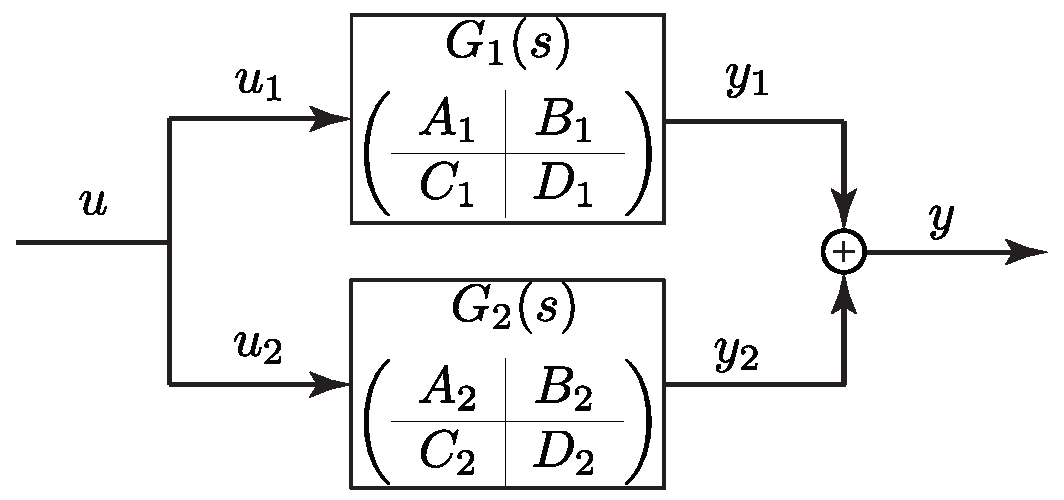
\includegraphics[width=0.70\textwidth]{parallel}
    \end{center}
  \end{minipage}
    \end{center}
		
The transfer function of the connection is simply equal to $G(s) = G_1(s) + G_2(s)$. Let $x_1$ and $x_2$
state-variables of the sub-systems, then natural choice of the state variable for the series connection is 
$x = \begin{bmatrix} x_1 \\ x_2 \end{bmatrix}$. Under this definition the state-space representation for the whole system 
can be found as
%
\begin{align*}
A = \left[ \begin{array}{c|c} A_1 & 0 \\ \hline 0  & A_2 \end{array} \right]
\, , \, B = \left[ \begin{array}{c} B_1 \\ \hline B_2   \end{array} \right]
\, , \, C = \left[ \begin{array}{c|c} C_1 & C_2  \end{array} \right]
\, , \, D = \left[ \begin{array}{c} D_1 +  D_2  \end{array} \right]
\end{align*}
%
Clearly eigenvalues of A are the combination of the eigenvalues of $A_1$ and $A_2$ and the poles of the system 
Let's analyze the observability of the connection via one of the modal reachability tests. 
%
\begin{align*}
	\left[ \begin{array}{c} \lambda I - A \\ \hline C \end{array} \right]
	= 
	\left[ \begin{array}{c|c} \lambda I - A_1 & 0 \\ \hline 0 &  \lambda I - A_2 \\ \hline 
	 C_1 & C_2
	\end{array} \right]
\end{align*}
%
It is easy to observe that combined system is always observable if $A_o1$ 
and $A_2$ does not share any common eigenvalue. Thus a necessary (but not sufficient) condition 
such that parallel connection loses observability is that $A_1$ and $A_2$ will have at least 1 
common eigenvalue. Let's assume that $\lambda_c$ is a common eigenvalue/pole of both sub-systems
Then $\left[ \begin{array}{c} \lambda I - A \\ \hline C \end{array} \right]_{\lambda = \lambda_c}$ 
looses rank, if $\exists v = \begin{bmatrix} v_1 \\ v_2 \end{bmatrix}$ such that 
%
%
\begin{align*}
	&\left[ \begin{array}{c} \lambda I - A \\ \hline C \end{array} \right] v  = 0 
	\, \iff \,  \left[ \begin{array}{c|c} \lambda I - A_1 & 0 \\ \hline 0 &  \lambda I - A_2 \\ \hline  C_1 & C_2 \end{array} \right] \begin{bmatrix} v_1 \\ v_2 \end{bmatrix} = 0
	\, \iff \, 
	\\
	&A_1 v_1 = \lambda_c v_1 \, , \, A_2 v_2 = \lambda_c v_2 \, , \& \, C_1 v_1 + C_2 v_2 = 0
\end{align*}
%
In other words combined system looses observability if and only if $\exists \, \lambda_c  \, , \, v_1 \, ,\& \, v_2$ such that 
$\lambda_c$ is a common eigenvalue of both systems, and there exists an $(v_1,v_2)$ eigenvector pair ($v_i$ is an eigenvector of $A_i$ associated with $\lambda_c$)
such that $C_1 v_1 + C_2 v_2 = 0$.

Now analyze the reachability of the connection via one of the modal reachability tests. 
%
\begin{align*}
	\left[ \begin{array}{c|c} \lambda I - A & B \end{array} \right]
	= 
	\left[ \begin{array}{c|c|c} \lambda I - A_1 & 0 & B_1 \\ \hline 0 &  \lambda I - A_2 & B_2 
	\end{array} \right]
\end{align*}
%
It is easy to observe that combined system is always reachable if $A_1$ 
and $A_2$ does not share any common eigenvalue. Thus a necessary (but not sufficient) condition 
such that parallel connection loses reahcability is that $A_1$ and $A_2$ will have at least 1 
common eigenvalue. Let's assume that $\lambda_c$ is a common eigenvalue/pole of both sub-systems
Then $\left[ \begin{array}{c|c} \lambda I - A & B \end{array} \right]_{\lambda = \lambda_c}$ 
looses rank, if $\exists w = \begin{bmatrix} w_1 \\ w_2 \end{bmatrix}$ such that 
%
%
\begin{align*}
	&w^T \left[ \begin{array}{c|c} \lambda_c I - A & B \end{array} \right] = 0 
	\, \iff \,  \begin{bmatrix} w_1^T & w_2^T \end{bmatrix} \left[ \begin{array}{c|c|c} \lambda_c I - A_1 & 0 & B_1  \\ \hline 0 &  \lambda_c I - A_2 & B_2 \end{array} \right]  = 0
	\, \iff \, 
	\\
	&w_1^T A_1 = \lambda_c w_1^T \, , \, w_2^T A_2 = \lambda_c w_2^T \, , \& \, w_1^T B_1 + w_2^T B_2 = 0
\end{align*}
%
In other words combined system looses reachability if and only if $\exists \, \lambda_c  \, , \, w_1 \, ,\& \, w_2$ such that 
$\lambda_c$ is a common eigenvalue of both systems, and there exists an $(w_1,w_2)$ left-eigenvector pair ($w_i$ is a left eigenvector of $A_i$ associated with $\lambda_c$)
such that $w_1^T B_1 + w_2^T B_2 = 0$.










% **** This ENDS THE EXAMPLES. DON'T DELETE THE FOLLOWING LINE:
\end{document}
